\documentclass[12pt,a4paper]{report}

\usepackage[margin=1in]{geometry}
\usepackage{setspace}
\usepackage{graphicx}
\usepackage{array}
\usepackage{booktabs}
\usepackage{longtable}
\usepackage{float}
\usepackage{titlesec}
\usepackage{tocloft}
\usepackage{hyperref}
\usepackage{xcolor}
\usepackage{tikz}
\usetikzlibrary{arrows.meta, positioning, shapes.geometric}

\onehalfspacing
\setlength{\parindent}{0pt}
\setlength{\parskip}{6pt}
\hypersetup{
    colorlinks=true,
    linkcolor=black,
    urlcolor=blue,
    citecolor=black
}

\titleformat{\chapter}{\normalfont\huge\bfseries}{Chapter \thechapter}{20pt}{\Huge}
\renewcommand{\contentsname}{Contents}

\begin{document}

\begin{titlepage}
    \begin{center}
        \vspace*{0.5cm}

        {\Large \textbf{KLE Technological University}}\\
        {\large Dr. M. S. Sheshgiri Campus, Belagavi, 590008}\\[0.3cm]
        {\large Department of Electronics and Communication Engineering}\\[1.0cm]

        {\Large \textbf{MINOR PROJECT REPORT}}\\[0.8cm]

        {\Huge \textbf{PCB Fault Detection and Reconstruction}}\\[0.4cm]
        {\Large \textbf{Using Generative AI and Computer Vision}}\\[1.0cm]

        {\large (Semester VI)}\\[0.2cm]
        {\large Course Code: \textbf{25EECW302}}\\[1.0cm]

        {\large \textbf{Submitted By}}\\[0.3cm]
        \begin{tabular}{>{\bfseries}l l}
            Student Name 1 & USN 1\\
            Student Name 2 & USN 2\\
            Student Name 3 & USN 3\\
            Student Name 4 & USN 4\\
        \end{tabular}\\[1.0cm]

        {\large \textbf{Under the Guidance of}}\\[0.3cm]
        {\large Prof. Guide Name}\\
        {\large Department of Electronics and Communication Engineering}\\[1.0cm]

        {\large KLE Technological University}\\
        {\large Dr. M. S. Sheshgiri Campus, Belagavi}\\[0.5cm]
        {\large Academic Year 2025--2026}
    \end{center}
\end{titlepage}

\pagenumbering{roman}
\tableofcontents
\clearpage
\pagenumbering{arabic}

\chapter{Introduction}

Printed Circuit Boards (PCBs) are the basic building blocks of almost all electronic systems. They provide mechanical support and electrical interconnection for electronic components such as resistors, capacitors, integrated circuits, connectors and sensors. The reliability of an electronic product depends greatly on the quality of the PCB and the correctness of its soldering, traces and component placement.

During manufacturing, assembly, repair or long-term usage, PCBs may develop several types of faults. Common defects include solder bridges, cold solder joints, missing components, burnt components, lifted pads, cracked boards, oxidation, delamination, open traces and short circuits. Manual inspection of PCBs is time-consuming and depends heavily on the skill and experience of the technician. In high-volume production or repair environments, manual inspection may also lead to inconsistent results.

This project titled \textbf{PCB Fault Detection and Reconstruction} proposes a Python-based web application that uses computer vision and generative artificial intelligence to assist PCB inspection. The system accepts a PCB image from the user, preprocesses it using OpenCV, analyzes it using a multimodal vision model and returns a structured fault report. In addition to fault detection, the system also generates a healthy-board reconstruction guide and provides a reconstructed image preview of the defect-free PCB.

The application is developed using Python, Streamlit, OpenCV, Pillow, NumPy and an AI vision API. Streamlit provides an interactive dashboard for uploading PCB images, viewing inspection results, reading reconstruction steps and downloading the reconstructed image. OpenCV is used for resizing, color conversion, contrast enhancement and local reconstruction preview generation.

The main objective of this project is to create an end-to-end tool that can support PCB quality inspection and repair guidance in a simple and user-friendly manner. The system does not replace a trained technician, but it provides a fast first-level inspection, defect summary, repair recommendation and healthy-board reference output.

\chapter{Literature Survey}

\section{Automated Optical Inspection for PCB Quality Control}

Automated Optical Inspection (AOI) systems are widely used in electronics manufacturing to detect visible defects on PCBs. These systems use image processing techniques to compare captured board images with reference templates. AOI systems are effective for detecting missing components, incorrect orientation, soldering defects and surface-level faults. However, traditional AOI systems often require controlled lighting, fixed camera setups and predefined board templates.

\section{Image Processing Based PCB Defect Detection}

Image processing techniques such as thresholding, edge detection, contour extraction, color segmentation and morphological operations are commonly used for PCB fault detection. These methods can identify cracks, dark burn marks, broken traces and solder irregularities. Although they are computationally efficient, purely rule-based image processing methods may fail when the PCB layout, lighting condition or defect appearance changes significantly.

\section{Machine Learning and Deep Learning in Visual Inspection}

Machine learning and deep learning methods have improved visual inspection accuracy by learning features directly from images. Convolutional Neural Networks (CNNs) are often used for classification and object detection tasks. They can classify defects and localize damaged regions when trained with sufficient labeled data. However, training such models requires a large dataset, careful annotation and significant computational resources.

\section{Generative AI for Visual Reasoning and Technical Explanation}

Recent multimodal generative AI models can accept images and text prompts together. Such models are capable of interpreting visual information and generating structured explanations. For this project, a multimodal vision model is used to inspect the uploaded PCB image and return a JSON-based fault analysis. The model is prompted to behave like an expert PCB quality control inspector and provide defect type, severity, location, description and recommended action.

\section{AI-Assisted Reconstruction and Repair Guidance}

PCB reconstruction requires understanding what a healthy board should look like after repair. Generative AI can help by producing step-by-step repair instructions, expected healthy conditions and a reference prompt for generating a defect-free board image. When direct AI image generation is unavailable due to quota limitations, local computer vision techniques such as inpainting and patch-based repair can be used to create an approximate reconstruction preview.

\chapter{Proposed System Architecture}

The proposed system is a web-based PCB inspection and reconstruction application. It consists of the following major modules:

\begin{itemize}
    \item Image Upload and Validation Module
    \item Image Preprocessing Module
    \item PCB Fault Detection Module
    \item Reconstruction Guidance Module
    \item Reconstructed Image Generation Module
    \item Streamlit Dashboard Module
\end{itemize}

The user uploads a PCB image in JPG or PNG format. The image is validated for file type and size. It is then preprocessed using OpenCV to improve visual clarity. The preprocessed image is sent to the AI vision model for fault detection. The model returns a structured JSON response containing PASS/FAIL status, defect list, severity, location, component analysis, quality score and summary.

For reconstruction, the same PCB image is analyzed again using a restoration-focused prompt. The system generates repair steps, healthy-board description, repair difficulty and a reference image prompt. A reconstructed image is then generated either through an image-generation model or through a local computer-vision fallback method.

\section{Input Parameters}

\begin{itemize}
    \item PCB image in JPG or PNG format
    \item API key for AI model access
    \item Selected analysis model
    \item Contrast enhancement option
\end{itemize}

\section{Output Parameters}

\begin{itemize}
    \item Overall PCB status: PASS or FAIL
    \item Confidence score
    \item List of detected defects
    \item Component-wise analysis
    \item Quality score from 0 to 100
    \item Reconstruction steps
    \item Healthy-board description
    \item Reconstructed PCB image preview
    \item Downloadable reconstructed image
\end{itemize}

\chapter{System Workflow}

The workflow of the proposed system begins with image upload. After validation, the image is resized and enhanced. The fault detection module analyzes the image and displays a structured report. The reconstruction module then generates repair guidance and a healthy-board reference. Finally, the reconstructed image generation module produces a visual preview of the repaired PCB.

\begin{figure}[H]
    \centering
    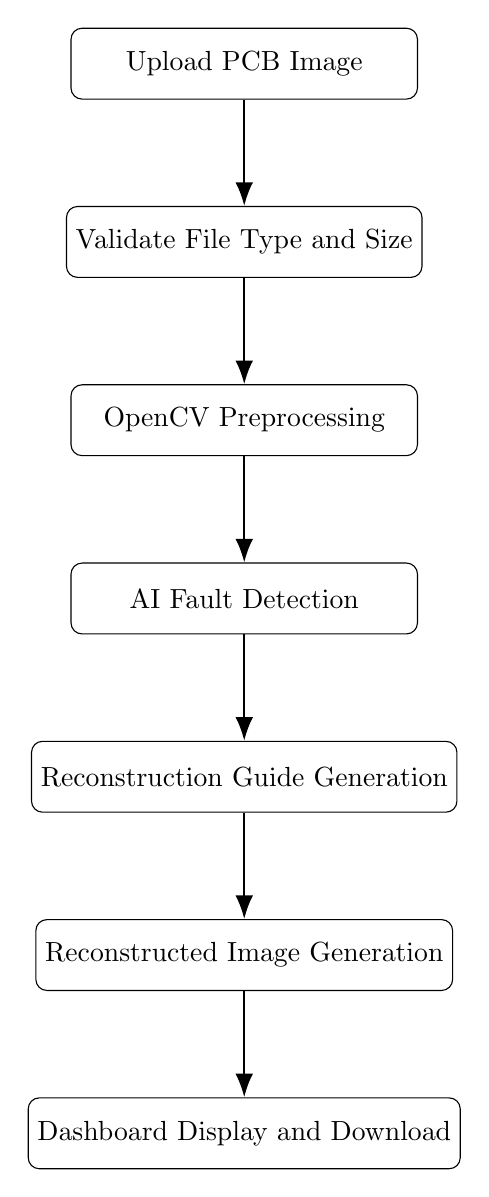
\begin{tikzpicture}[
        node distance=1.35cm,
        block/.style={rectangle, draw, rounded corners, align=center, minimum width=4.4cm, minimum height=0.9cm},
        arrow/.style={-{Latex[length=3mm]}, thick}
    ]
        \node[block] (upload) {Upload PCB Image};
        \node[block, below=of upload] (validate) {Validate File Type and Size};
        \node[block, below=of validate] (preprocess) {OpenCV Preprocessing};
        \node[block, below=of preprocess] (detect) {AI Fault Detection};
        \node[block, below=of detect] (guide) {Reconstruction Guide Generation};
        \node[block, below=of guide] (image) {Reconstructed Image Generation};
        \node[block, below=of image] (dashboard) {Dashboard Display and Download};

        \draw[arrow] (upload) -- (validate);
        \draw[arrow] (validate) -- (preprocess);
        \draw[arrow] (preprocess) -- (detect);
        \draw[arrow] (detect) -- (guide);
        \draw[arrow] (guide) -- (image);
        \draw[arrow] (image) -- (dashboard);
    \end{tikzpicture}
    \caption{Functional Flow Diagram of PCB Fault Detection and Reconstruction System}
\end{figure}

\chapter{Image Preprocessing}

Image preprocessing is an important stage because the quality of the input image directly affects the inspection result. The uploaded PCB image may have different dimensions, brightness levels, contrast values and color formats. Therefore, preprocessing is performed before sending the image for analysis.

The preprocessing module performs the following operations:

\begin{itemize}
    \item File validation for JPG and PNG formats
    \item Maximum file size check of 10 MB
    \item Image decoding using Pillow
    \item RGB conversion
    \item Resizing if the image is larger than 1024 pixels
    \item Contrast enhancement using CLAHE in LAB color space
    \item Re-encoding the processed image for model input
\end{itemize}

Contrast Limited Adaptive Histogram Equalization (CLAHE) is applied on the L channel of the LAB image. This improves the visibility of traces, solder joints and burnt regions without strongly distorting the color information of the PCB.

\chapter{PCB Fault Detection Module}

The PCB fault detection module analyzes the uploaded board image and returns a structured quality report. The model is instructed to behave like an experienced PCB quality control inspector. The response is restricted to JSON format so that the application can parse and display the results reliably.

The detection module identifies common PCB defects such as:

\begin{itemize}
    \item Solder bridge
    \item Cold solder joint
    \item Missing component
    \item Lifted pad
    \item PCB crack
    \item Burnt component
    \item Misaligned component
    \item Excess solder
    \item Insufficient solder
    \item Oxidation
    \item Delamination
    \item Open circuit trace
    \item Short circuit
\end{itemize}

The structured output generated by the module includes:

\begin{itemize}
    \item Overall status
    \item Confidence score
    \item Defects found
    \item Defect severity
    \item Defect location
    \item Recommended repair action
    \item Component analysis
    \item Quality score
    \item Summary
\end{itemize}

\chapter{Reconstruction Guidance Module}

The reconstruction guidance module uses the same uploaded PCB image and generates a detailed explanation of how the healthy version of the board should appear. This module is designed to support technicians during inspection and repair.

The reconstruction guide contains:

\begin{itemize}
    \item Identified board type
    \item Step-by-step repair procedure
    \item Area of the board requiring repair
    \item Action to be performed
    \item Expected result after repair
    \item Tools and materials required
    \item Healthy-board description
    \item Repair difficulty level
    \item Reconstruction summary
\end{itemize}

The repair steps are displayed as an interactive checklist in the dashboard. This allows users to mark completed repair steps while following the guide.

\chapter{Reconstructed Image Generation}

The reconstructed image generation module provides a visual representation of the expected healthy PCB. This is an important addition because the project title includes both fault detection and reconstruction. A text-only guide is useful, but a visual reconstructed image helps the user understand the expected final board appearance more clearly.

The system uses two methods for reconstructed image generation:

\section{AI Image Generation}

When image-generation quota is available, the system sends the healthy-board reference prompt to an image-capable AI model. The model generates a clean top-down reference image of the repaired PCB. The prompt instructs the model to preserve the board type, component density, trace structure, board color and technical appearance while removing visible defects.

\section{Local Computer Vision Reconstruction Preview}

If image-generation quota is not available, the application creates a local reconstruction preview using OpenCV. This fallback method detects dark burnt or damaged regions and attempts to repair them using patch-based reconstruction and inpainting.

The local reconstruction preview performs the following steps:

\begin{itemize}
    \item Detect dark scorch-like damaged regions
    \item Estimate valid PCB board surface regions
    \item Search for a clean donor patch from nearby board areas
    \item Blend the clean patch into the damaged region
    \item Apply inpainting to smooth remaining seams
    \item Sharpen and color-balance the final preview
\end{itemize}

The AI-generated image is preferred when available. The local preview is used as a backup so that the application can still provide a reconstructed image output even when external image generation is unavailable.

\chapter{Dashboard Design}

The dashboard is developed using Streamlit. It provides a simple and interactive interface for PCB inspection and reconstruction. The application is divided into three main tabs:

\begin{itemize}
    \item Dashboard
    \item Fault Detection
    \item Reconstruction Guide
\end{itemize}

\section{Dashboard Tab}

The dashboard tab shows the current status of the application. It displays image readiness, AI engine configuration, quality score, reconstructed image status, current PCB metadata, inspection status, defect severity breakdown and session activity.

\section{Fault Detection Tab}

The fault detection tab displays the uploaded PCB image on the left side and the analysis results on the right side. The results include PASS/FAIL badge, quality score progress bar, defect cards and component analysis table.

\section{Reconstruction Guide Tab}

The reconstruction guide tab displays the uploaded image, repair difficulty, board type, reconstruction checklist, healthy-board description, reference image prompt and reconstructed PCB image. The reconstructed image can also be downloaded.

\chapter{Implementation Environment}

The following tools and technologies were used for implementation:

\begin{itemize}
    \item Python 3.10+
    \item Streamlit
    \item OpenCV
    \item Pillow
    \item NumPy
    \item Python dotenv
    \item Google Generative AI SDK
    \item Google GenAI SDK for image generation
    \item Windows operating system
    \item Localhost deployment
\end{itemize}

The complete project is implemented as a Python web application. The application runs locally on port 8501 using Streamlit. A startup script is also provided so that the server can start automatically after user login.

\chapter{Implementation Details}

The project contains the following major files:

\begin{table}[H]
    \centering
    \begin{tabular}{p{5cm} p{9cm}}
        \toprule
        \textbf{File Name} & \textbf{Description}\\
        \midrule
        app.py & Main Streamlit application and dashboard layout\\
        detector.py & Fault detection prompt and response normalization\\
        reconstructor.py & Reconstruction guide prompt and response normalization\\
        gemini\_client.py & AI API wrapper, JSON parsing and image generation logic\\
        image\_utils.py & Image validation, preprocessing and local reconstruction preview\\
        ui\_components.py & Reusable UI components such as badges, cards and tables\\
        requirements.txt & List of Python dependencies\\
        .env.example & Example environment variable file for API key setup\\
        start\_dashboard.ps1 & PowerShell script to start the local dashboard\\
        start\_dashboard.bat & Windows batch launcher for automatic startup\\
        \bottomrule
    \end{tabular}
    \caption{Project File Structure}
\end{table}

The application follows a modular design so that each function is separated according to its responsibility. This improves readability, debugging and future expansion.

\chapter{Results and Testing}

The application was tested with PCB images containing visible board-level defects. The system successfully uploaded the image, performed preprocessing and displayed the image in the dashboard. Fault analysis generated structured results including board status, quality score, defect description and repair recommendation.

\section{Functional Test Cases}

\begin{table}[H]
    \centering
    \begin{tabular}{p{4cm} p{5cm} p{4cm} p{2cm}}
        \toprule
        \textbf{Test Case} & \textbf{Input} & \textbf{Expected Output} & \textbf{Status}\\
        \midrule
        Image upload & JPG or PNG PCB image & Image accepted and preview shown & Verified\\
        File validation & File above 10 MB & Error message displayed & Verified\\
        Preprocessing & Large PCB image & Resized and contrast enhanced image & Verified\\
        Fault detection & Faulty PCB image & JSON fault report displayed & Verified\\
        Defect cards & Detected defect list & Expandable severity cards & Verified\\
        Reconstruction guide & Faulty PCB image & Repair steps and healthy description & Verified\\
        Reconstructed image & Reference prompt & Generated or local preview image & Verified\\
        Download option & Reconstructed image & PNG image downloaded & Verified\\
        \bottomrule
    \end{tabular}
    \caption{Functional Test Case Verification}
\end{table}

\section{Observed Output}

The dashboard displays:

\begin{itemize}
    \item Uploaded PCB image
    \item PASS or FAIL status
    \item Quality score
    \item Defect severity breakdown
    \item Component analysis table
    \item Reconstruction checklist
    \item Healthy-board description
    \item Reconstructed image preview
    \item Download button for reconstructed image
\end{itemize}

The results confirm that the system provides both analysis and reconstruction support in a single application.

\chapter{Performance Comparison}

The proposed system improves over manual PCB inspection by providing fast visual analysis, structured reporting and repair guidance.

\begin{table}[H]
    \centering
    \begin{tabular}{p{4cm} p{5cm} p{5cm}}
        \toprule
        \textbf{Parameter} & \textbf{Manual Inspection} & \textbf{Proposed System}\\
        \midrule
        Inspection speed & Slower and technician-dependent & Faster first-level analysis\\
        Report format & Manual notes & Structured JSON-based report\\
        Defect severity & Subjective & Categorized as LOW, MEDIUM, HIGH or CRITICAL\\
        Reconstruction support & Depends on technician experience & Step-by-step repair guide\\
        Visual reference & Usually unavailable & Reconstructed image preview\\
        Repeatability & Varies by inspector & More consistent prompt-based analysis\\
        Dashboard & Not available & Interactive web dashboard\\
        \bottomrule
    \end{tabular}
    \caption{Comparison Between Manual Inspection and Proposed System}
\end{table}

\chapter{Applications}

The proposed system can be used in:

\begin{itemize}
    \item PCB manufacturing inspection
    \item Electronics repair laboratories
    \item Academic electronics laboratories
    \item Quality control departments
    \item Prototype board verification
    \item Embedded system development labs
    \item Training students in PCB defect identification
    \item Maintenance of electronic equipment
\end{itemize}

\chapter{Advantages of Proposed System}

\begin{itemize}
    \item Simple web-based dashboard
    \item Supports JPG and PNG PCB images
    \item Automatic image preprocessing
    \item Structured fault detection report
    \item Severity-based defect classification
    \item Component-wise analysis
    \item Step-by-step reconstruction guidance
    \item Reconstructed PCB image preview
    \item Downloadable reconstructed image
    \item Local fallback when image-generation quota is unavailable
    \item Easy to deploy locally using Streamlit
\end{itemize}

\chapter{Limitations}

The system has some limitations:

\begin{itemize}
    \item Accuracy depends on image quality and lighting
    \item Very small defects may not be detected clearly
    \item AI-generated results require verification by a human technician
    \item Image generation depends on API quota availability
    \item Local reconstruction preview is approximate and may not fully restore complex PCB layouts
    \item The system does not perform electrical continuity testing
\end{itemize}

\chapter{Conclusion}

This project presented the design and implementation of a PCB Fault Detection and Reconstruction application using Python, computer vision and generative AI. The system accepts a PCB image, preprocesses it using OpenCV and performs AI-based fault detection to generate a structured quality report.

The application identifies possible defects, assigns severity levels, provides component-wise analysis and recommends repair actions. In addition to detection, the system generates a reconstruction guide that explains how the healthy PCB should look and what steps are required for repair.

To support the reconstruction objective, the system also provides a reconstructed PCB image. When AI image-generation quota is available, the system can generate a healthy-board reference image. When quota is unavailable, the application creates a local computer-vision based reconstruction preview using patch repair and inpainting.

The complete system is deployed as a Streamlit dashboard and runs locally on the user's computer. The project demonstrates how AI and image processing can be combined to assist PCB quality inspection, repair planning and visual reconstruction.

\chapter{Future Scope}

Future improvements can include:

\begin{itemize}
    \item Training a custom PCB defect detection model
    \item Adding bounding boxes around detected defects
    \item Creating a dataset of faulty and healthy PCB images
    \item Improving reconstructed image quality using dedicated image restoration models
    \item Integrating electrical test results with visual inspection
    \item Supporting batch inspection of multiple PCB images
    \item Adding PDF report generation from inspection results
    \item Deploying the application on a local network server
    \item Adding role-based access for lab technicians and students
    \item Integrating camera capture for real-time PCB inspection
\end{itemize}

\end{document}
